%%%%%%%%%%%%%%%%%%%%%%%%%%%%%%%%%%%%%%%%%%%%%%%%%%%%%%%%%%%%%%%%%
\chapter{SIMULATION ENVIRONMENT}\label{ch:simulation_environment}
%%%%%%%%%%%%%%%%%%%%%%%%%%%%%%%%%%%%%%%%%%%%%%%%%%%%%%%%%%%%%%%%%

A discrete event simulator is developed in Python to study the effects of various spreading factor strategies in LoRaWANs. LoRaWAN spreading factor simulation tool source code is available at GitHub \cite{tugrul_yatagan_simlorasf}. Simulation tool supports custom LoRaWAN topologies as well as randomly generated LoRaWAN topologies. Simulator can generate uniformly distributed circular shape network topology with following input parameters: radius (r) in meter (m), number of nodes and number of gateways. Global simulation input parameters are simulation duration in second (s), packet size in Byte (B), packet generation rate in packets per second (pps) and spreading factor assignment method. With these inputs, the simulator produces total number of generated packets, number of successfully received packets, number of interfered packets, number of under sensitivity packets, network packet delivery ratio percentage (PDR), network throughput in bits per second (bps) and total transmit energy consumption in Joule (J). Simulator also produces prediction accuracy percentage and confusion matrix for machine learning schemes. 

The simulation tool LoRaWAN network gateway placement for various number of gateways can be found in Figure in Figure \ref{fig:topology}. Simulation tool first places gateways by number of gateways input. The tool homogeneously distributes gateways over network by keeping them apart as possible. Then the tool randomly places end nodes in  network radius.

\begin{figure}
\centering
\subfigure[Singe gateway]{
\label{fig:1_gw_topology}
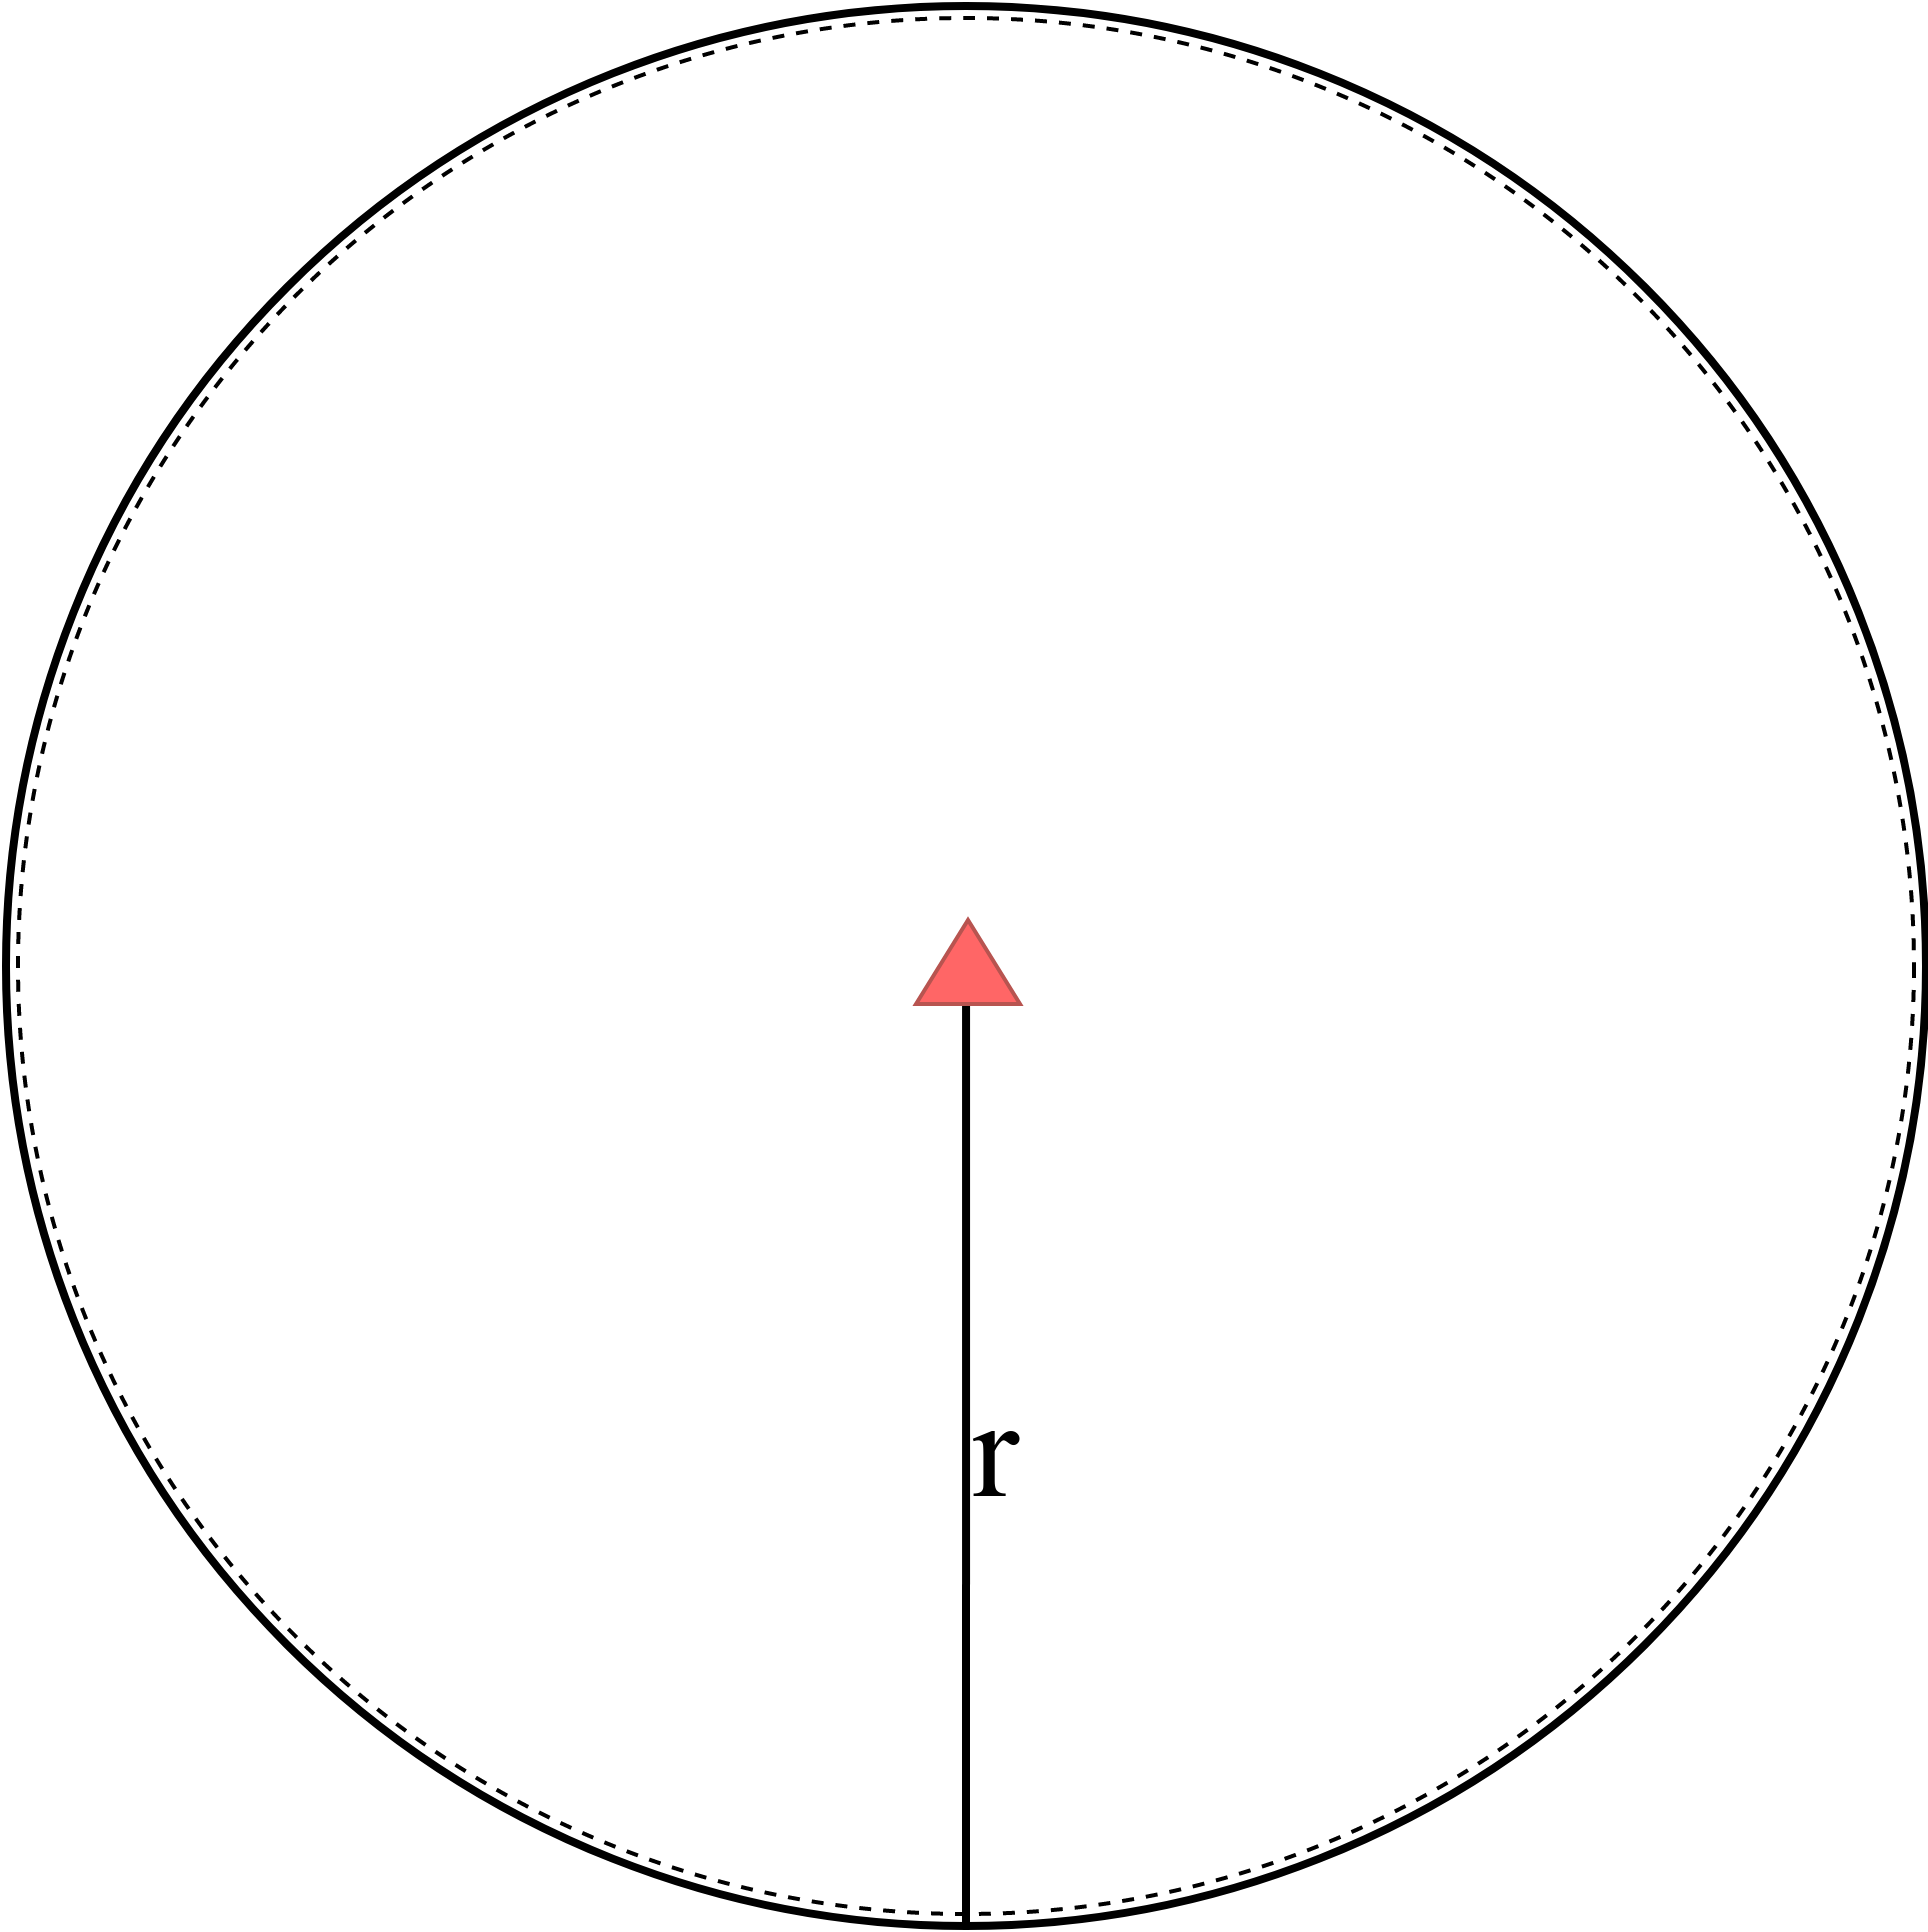
\includegraphics[width=.46\linewidth]{{fig/lora_1_gw_topology}.png}}
\qquad
\subfigure[Dual gateway]{
\label{fig:2_gw_topology}
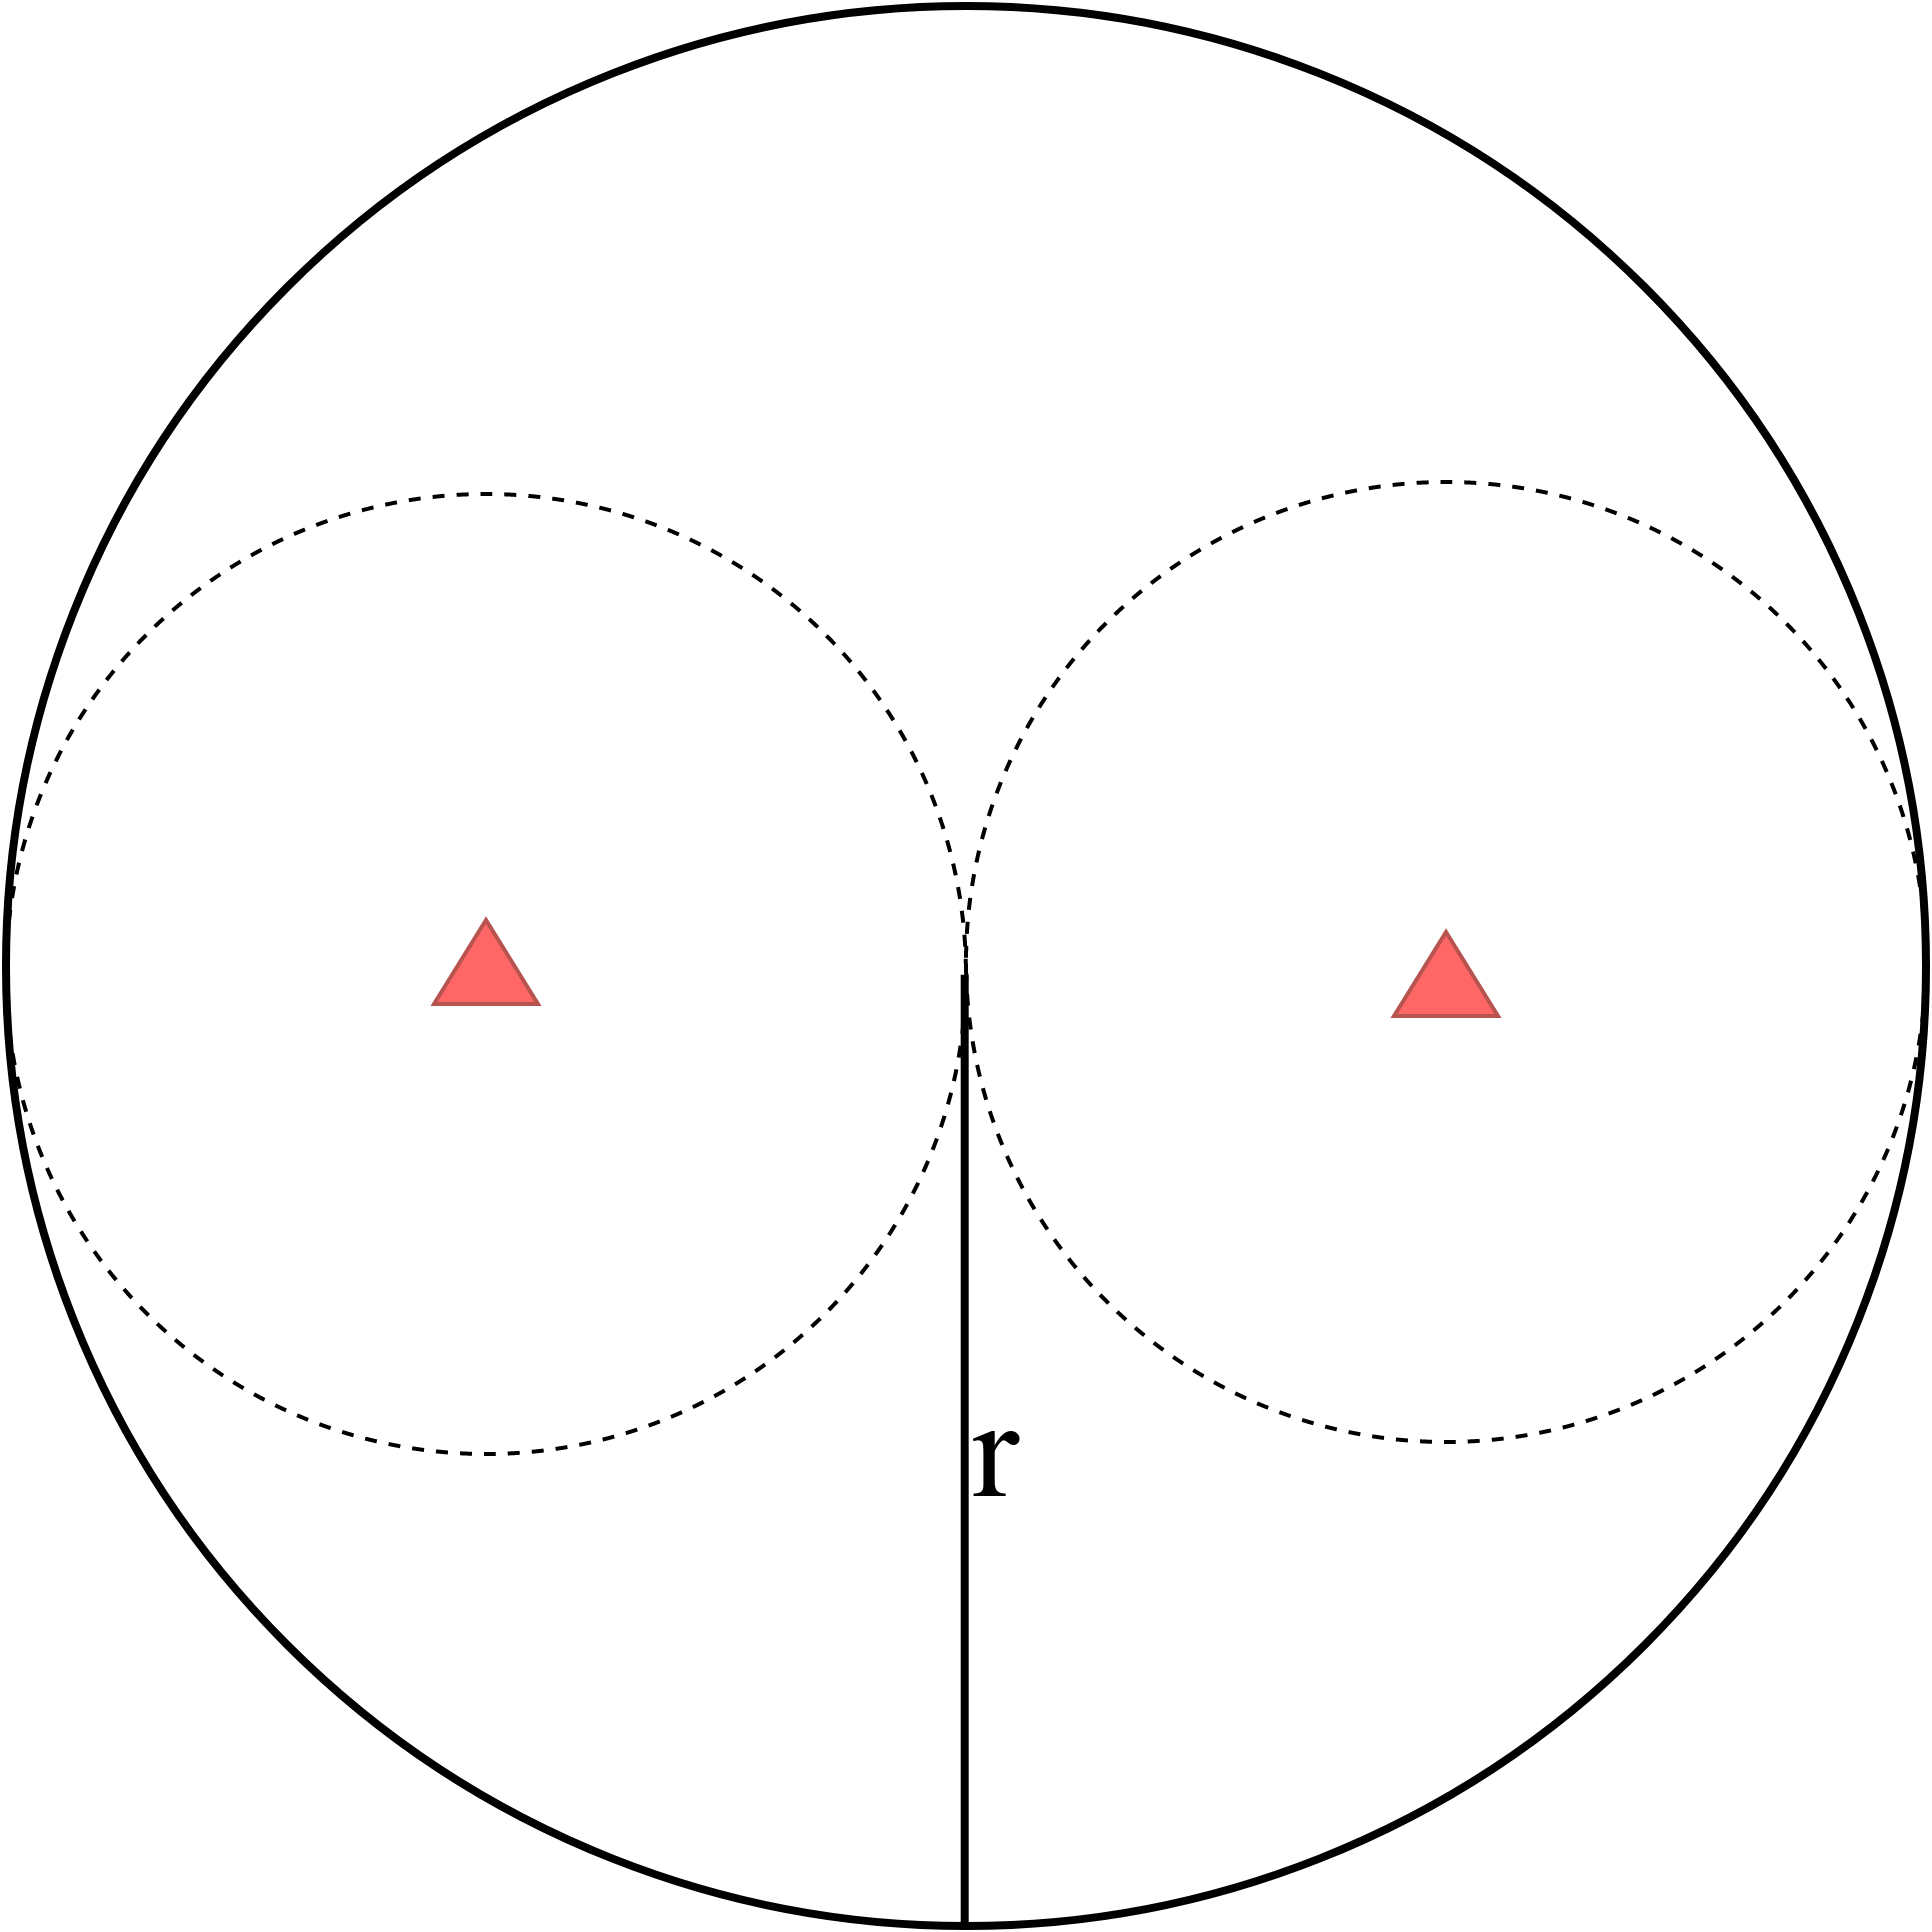
\includegraphics[width=.46\linewidth]{{fig/lora_2_gw_topology}.png}}  \\
\subfigure[Triple gateway]{
\label{fig:3_gw_topology}
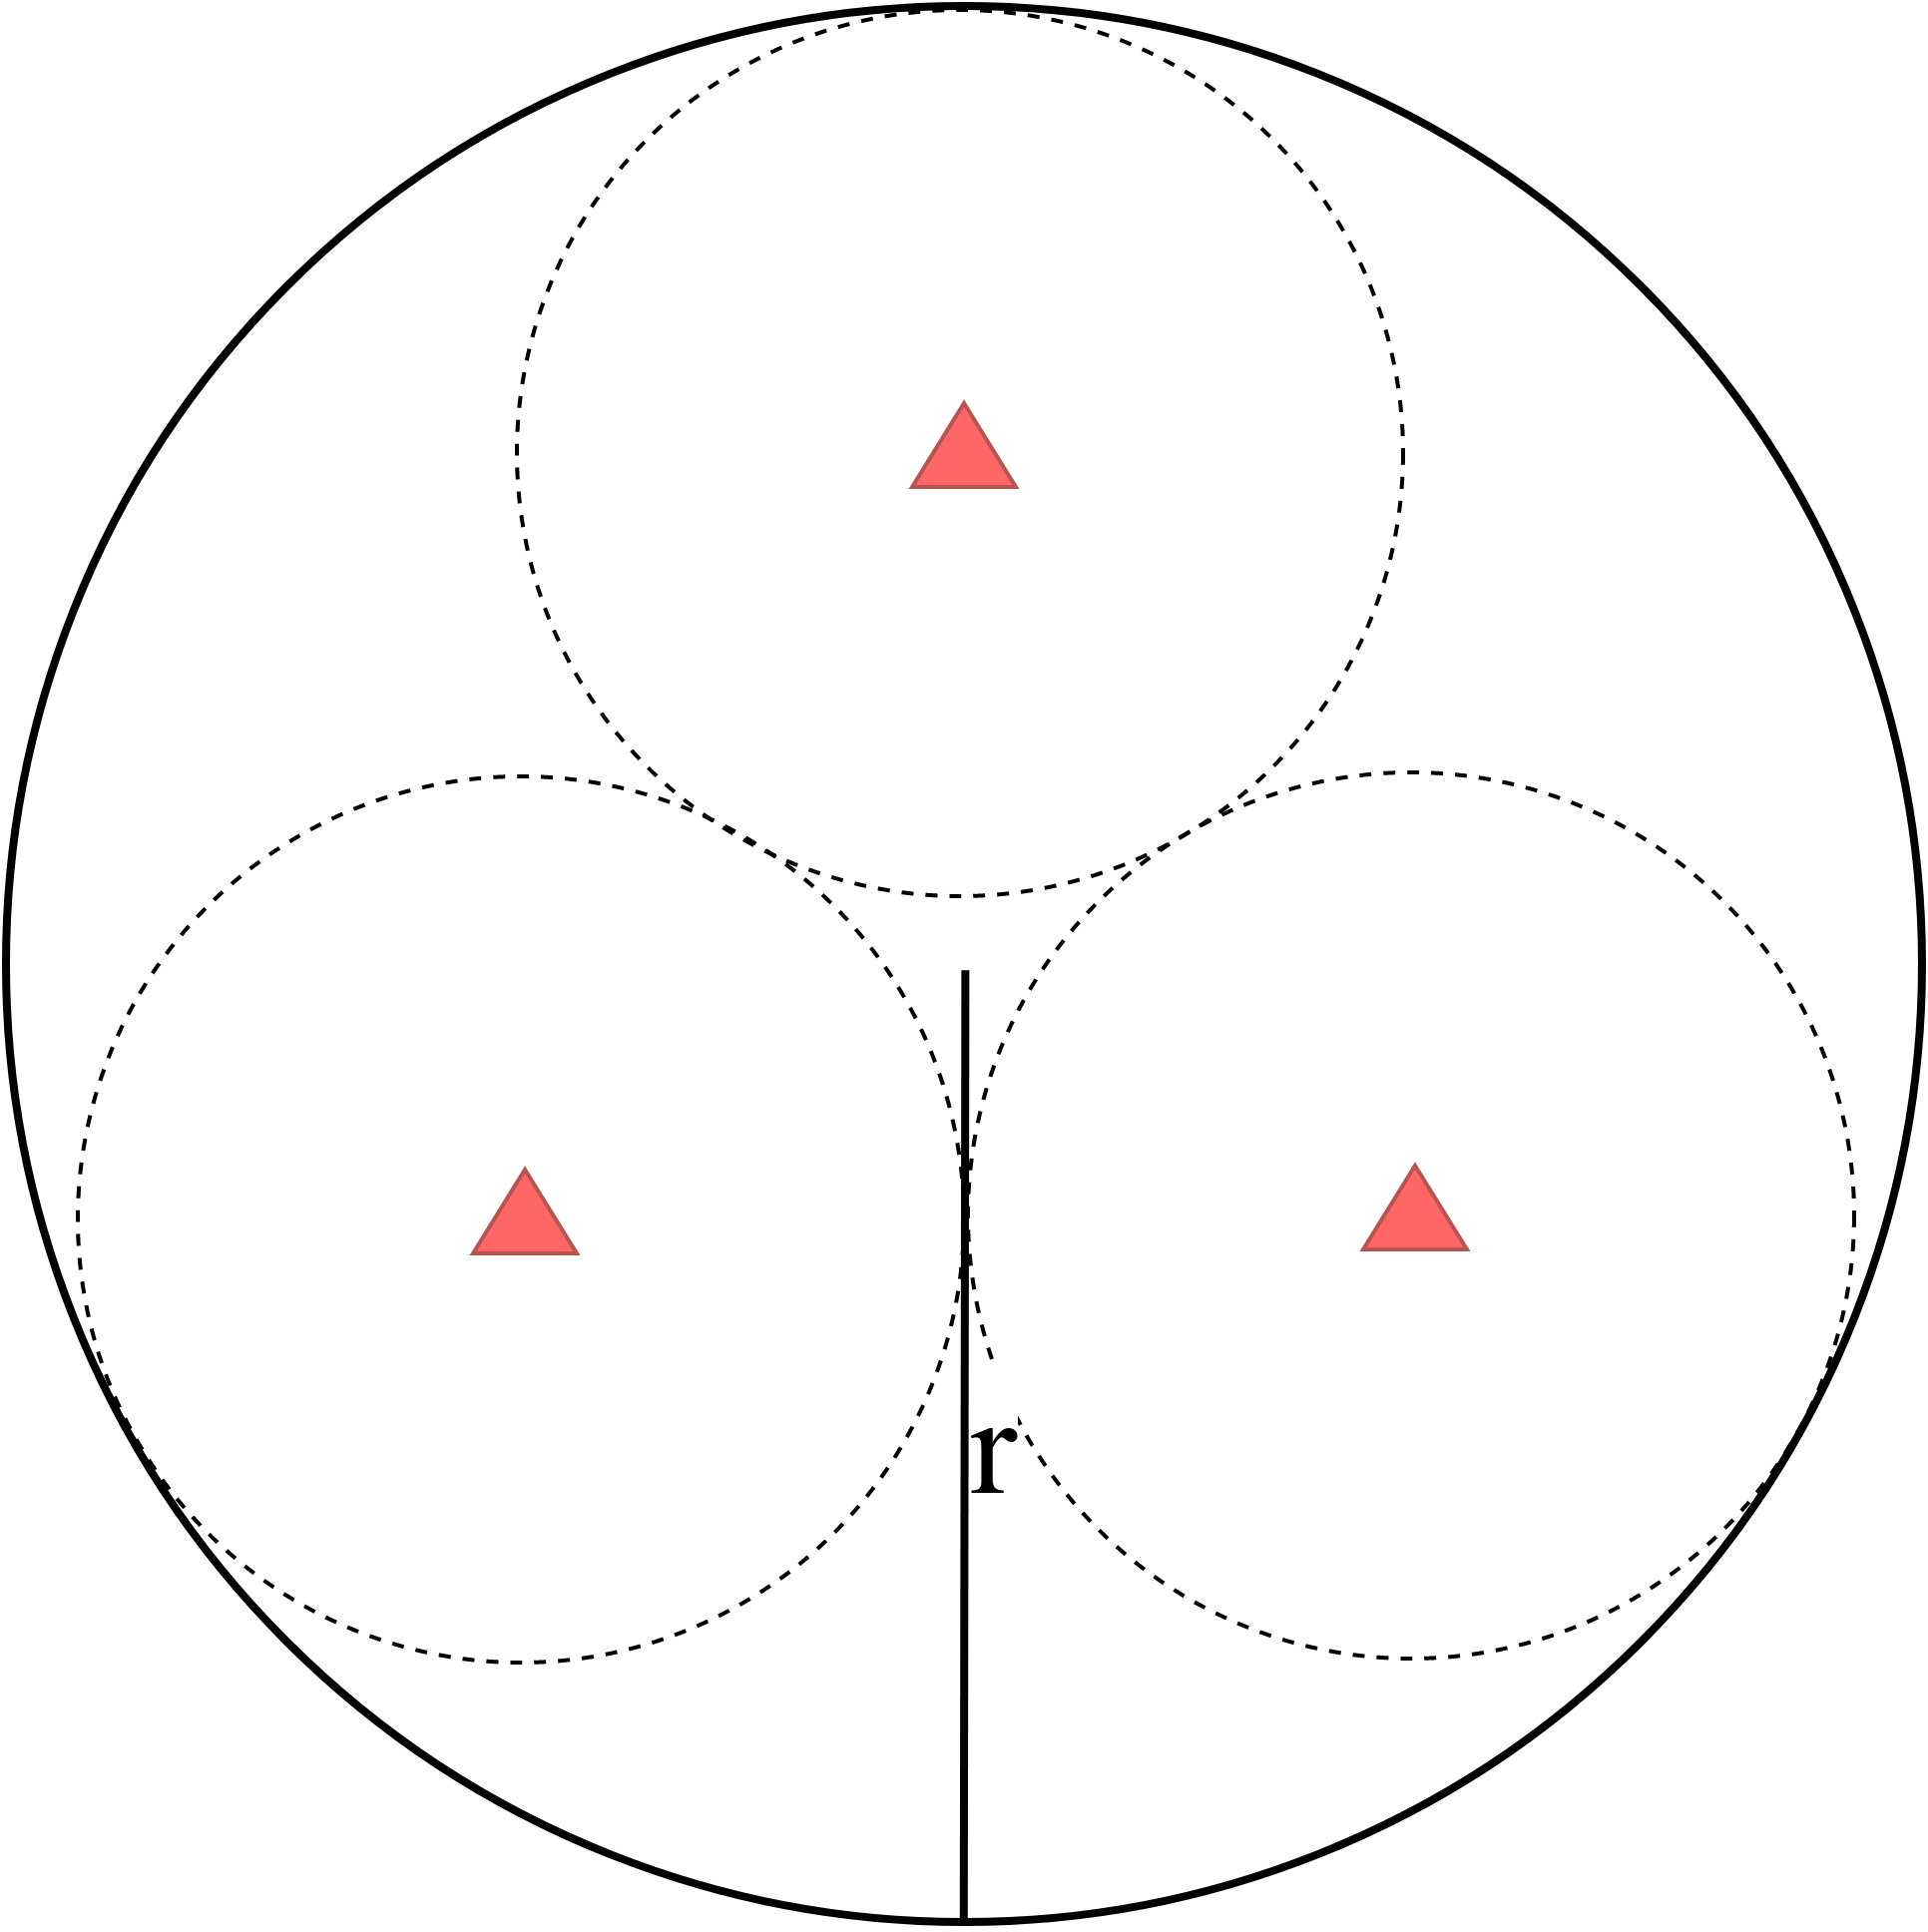
\includegraphics[width=.46\linewidth]{{fig/lora_3_gw_topology}.png}}
\qquad
\subfigure[Quad gateway]{
\label{fig:4_gw_topology}
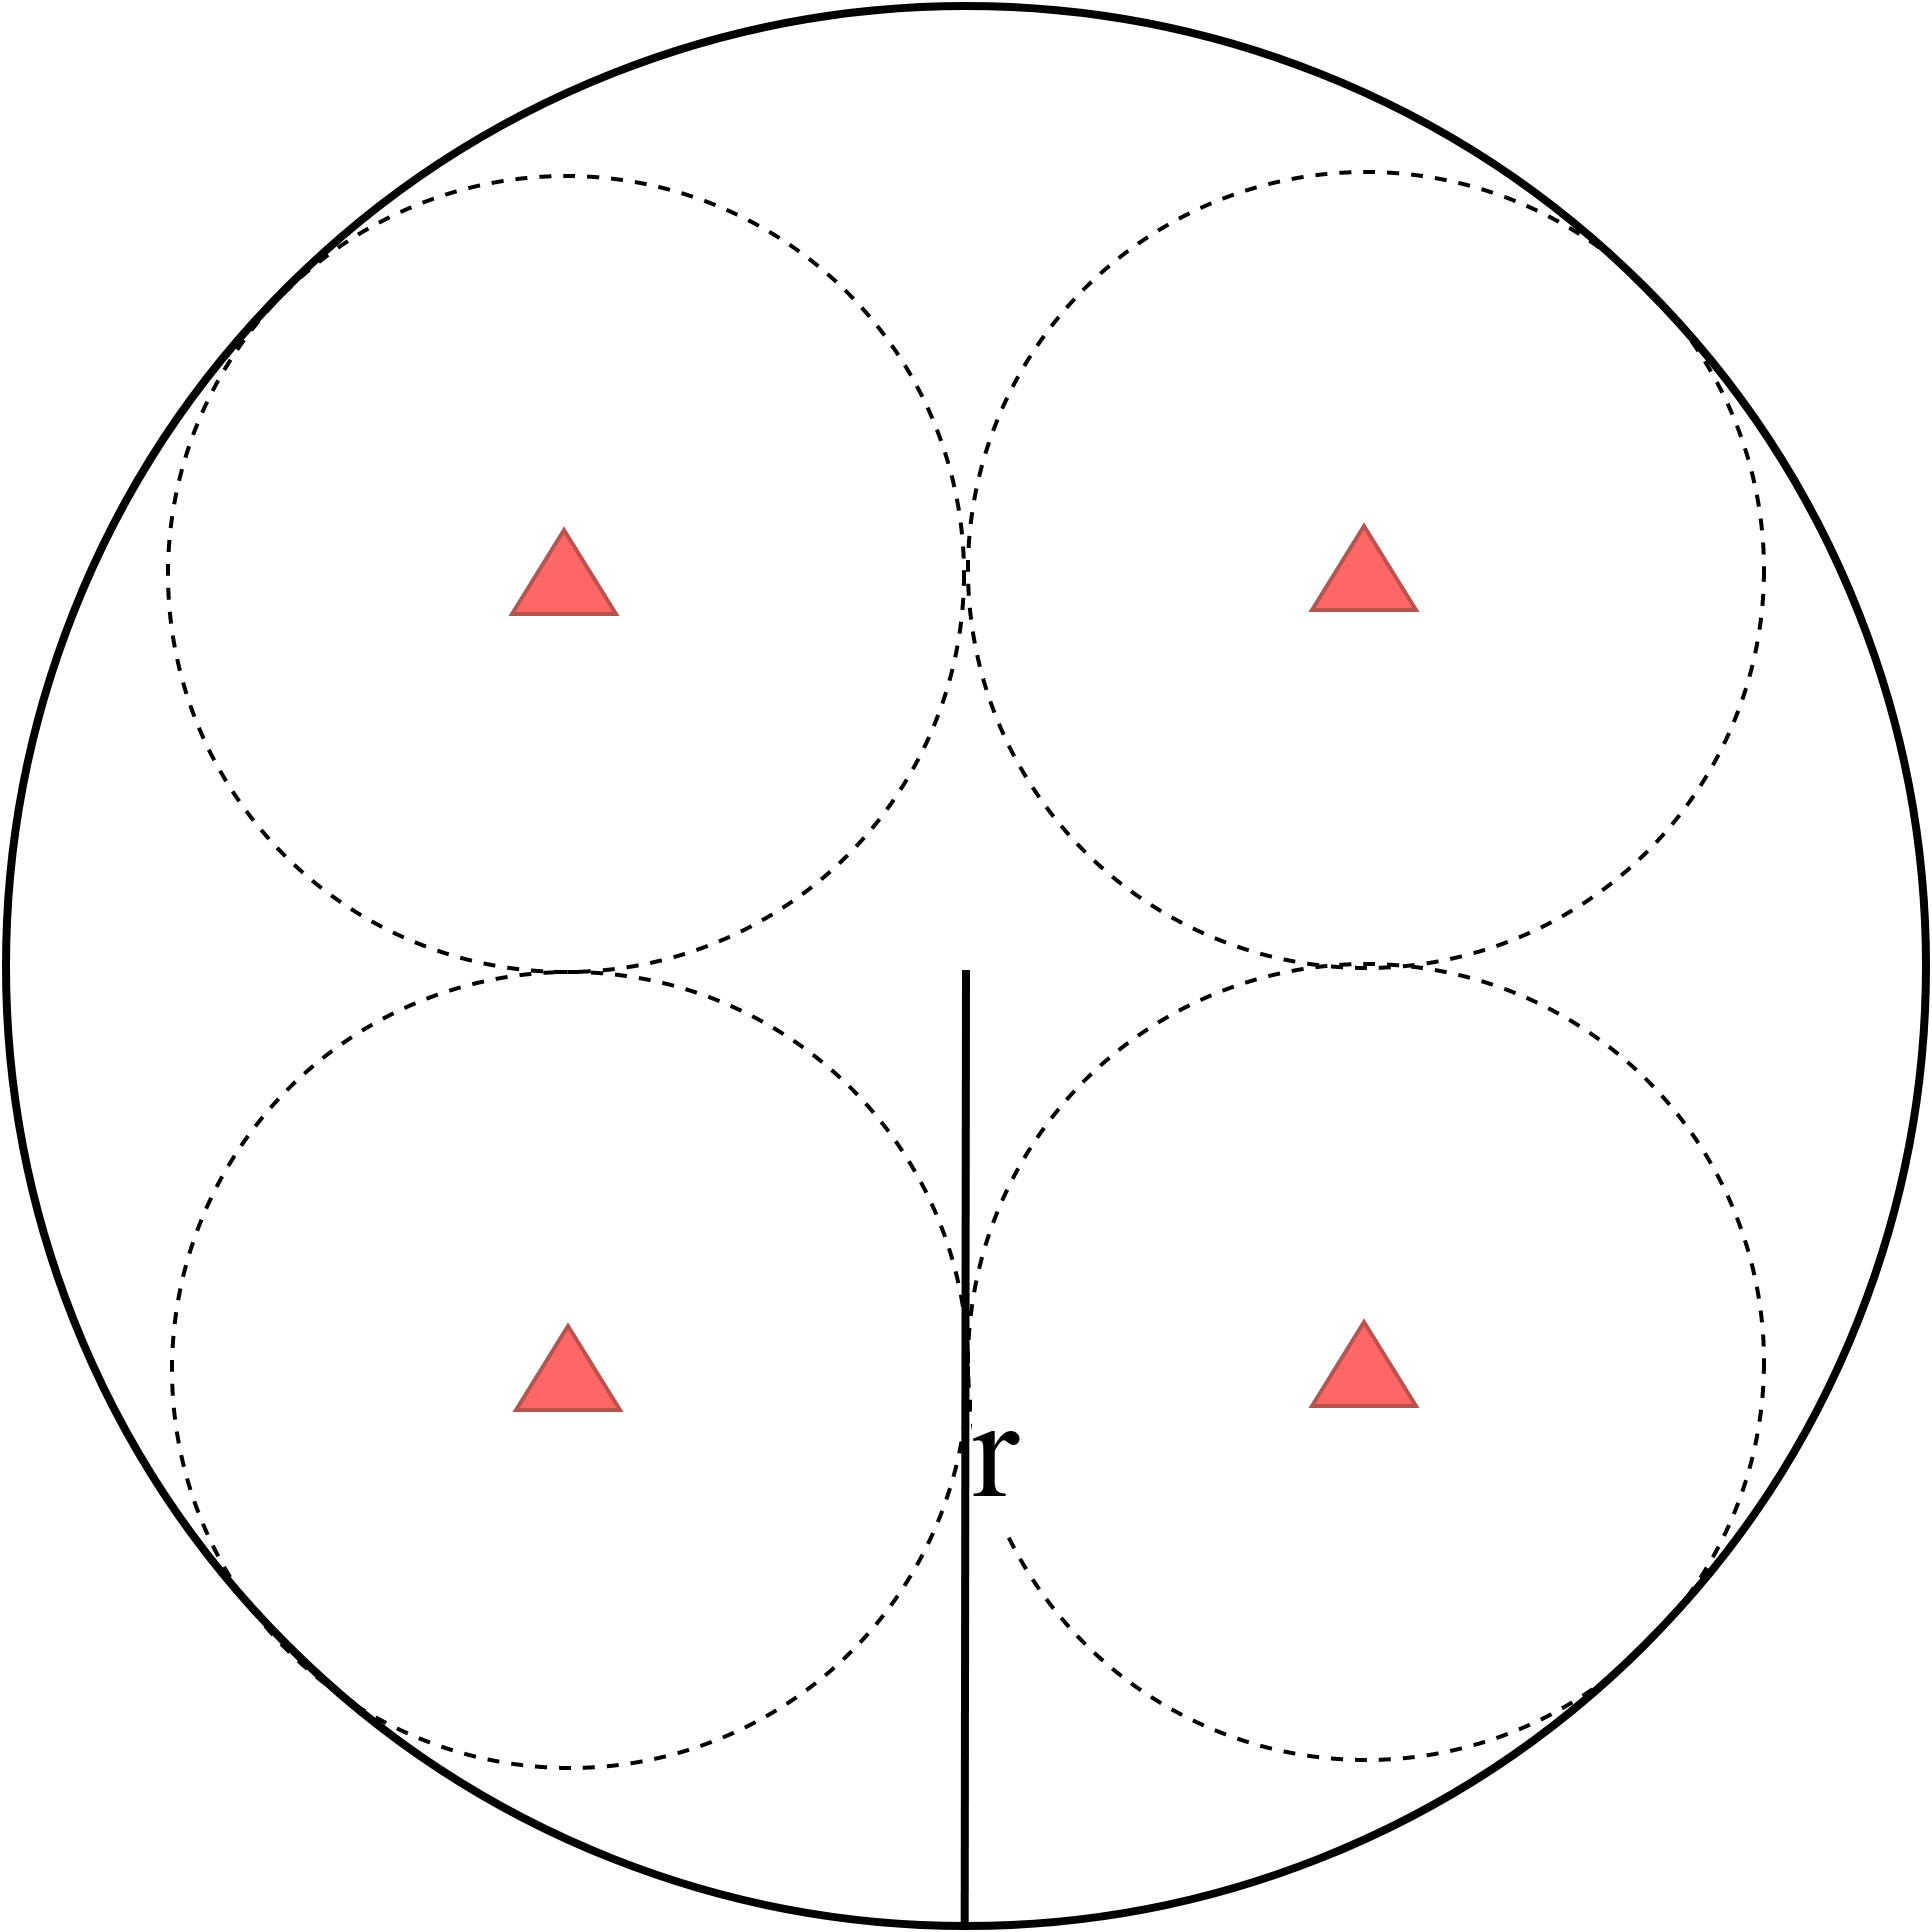
\includegraphics[width=.46\linewidth]{{fig/lora_4_gw_topology}.png}}
\vspace*{4mm}
\caption{Network topologies for various number of gateways.}
\label{fig:topology}
\end{figure}

The simulation tool only covers the LoRaWAN Class A devices since Class A behaviour is the default operation mode and Class A behavior leads to the lowest power consumption. Transmissions are always initiated by end nodes in pure ALOHA manner. Nodes generate a new packet for given packet rate parameter. Packets can be generated according to Poisson interval or periodic interval.

Timing diagram for periodic traffic generation is shown in Figure \ref{fig:lora_traffic_periodic}. Initial transmission intervals are always generated by Poisson as it can be seen in first transmission in Figure \ref{fig:lora_traffic_periodic}. This prevents continuous collisions between periodic transmissions by adding various time gap between different nodes. $1/\lambda$ represents periodic traffic generation interval between two transmission for traffic rate input ($\lambda$). $f(\lambda)$ represents Poisson traffic generation interval for traffic rate input \cite{probability}.

Timing diagram for Poisson traffic generation is shown in Figure \ref{fig:lora_traffic_poisson}. All transmission intervals are generated according to Poisson for given packet rate parameter.

\begin{figure}
\centering
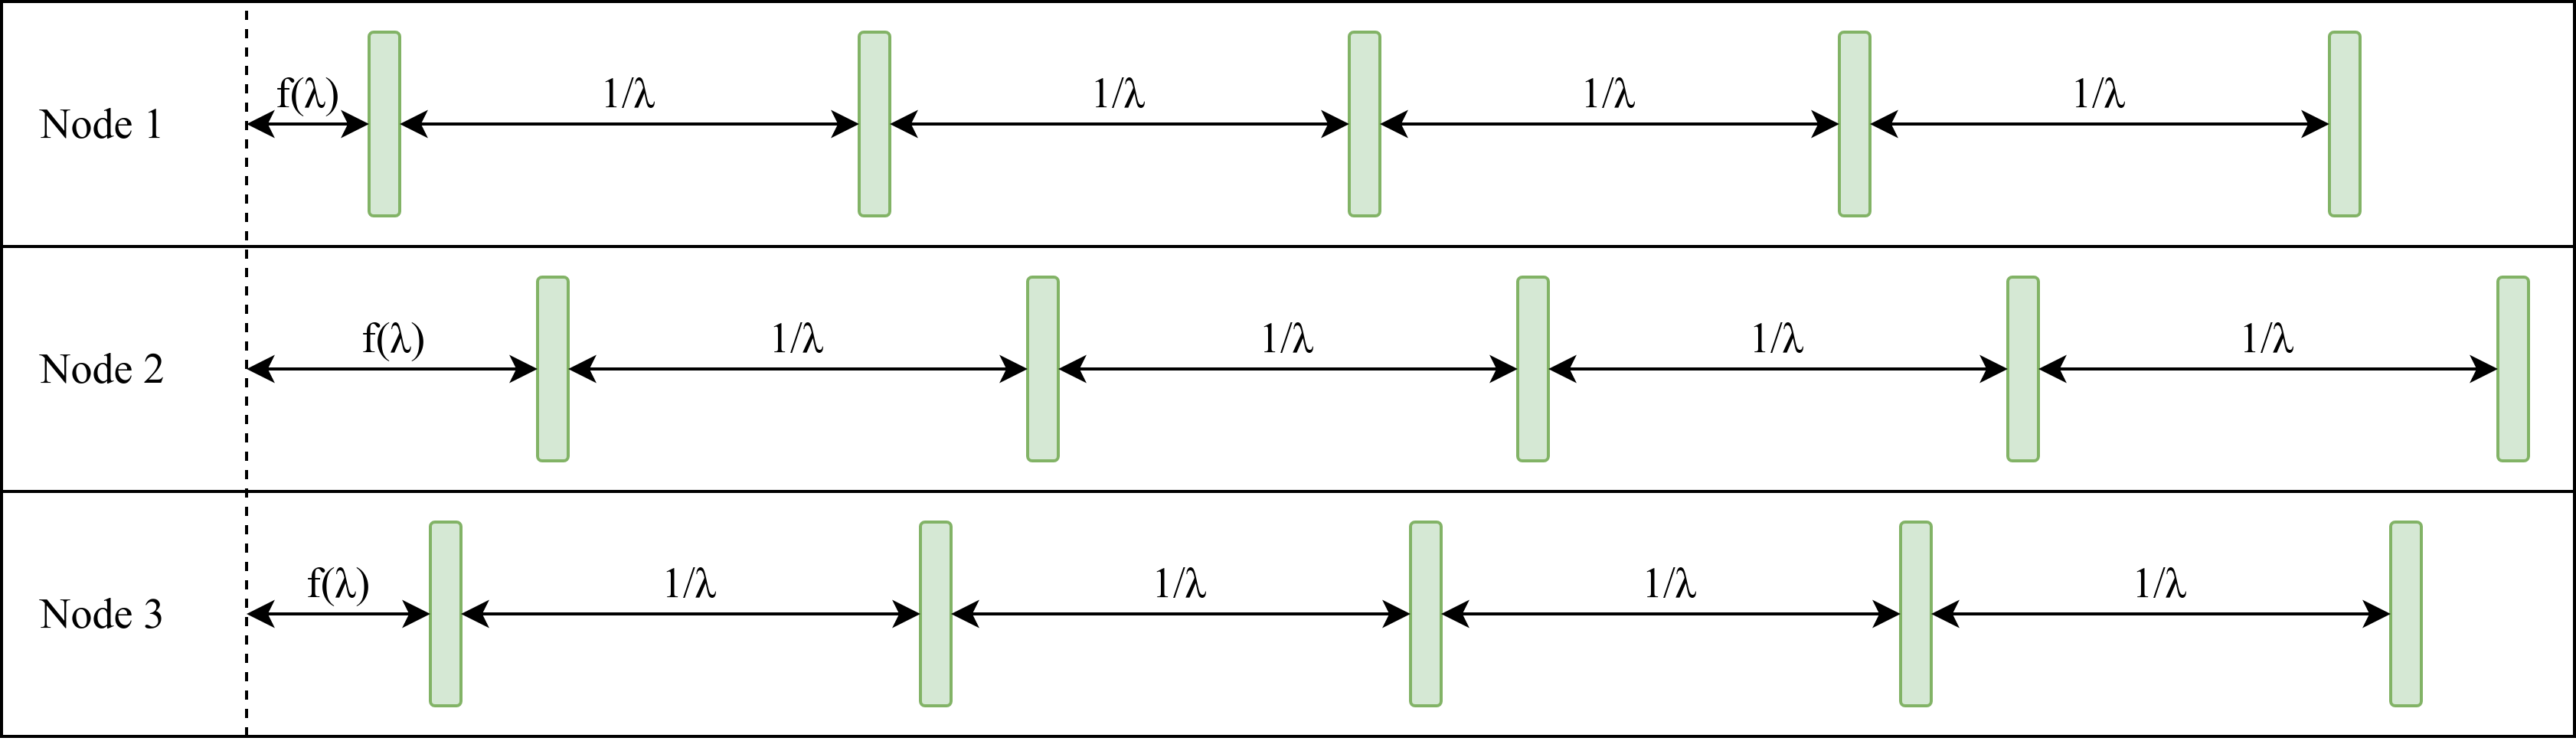
\includegraphics[width=\linewidth]{{fig/lora_traffic_periodic}.png}
\vspace*{2mm}
\caption{Periodic traffic generation timing diagram.}
\label{fig:lora_traffic_periodic}
\end{figure}

\begin{figure}
\centering
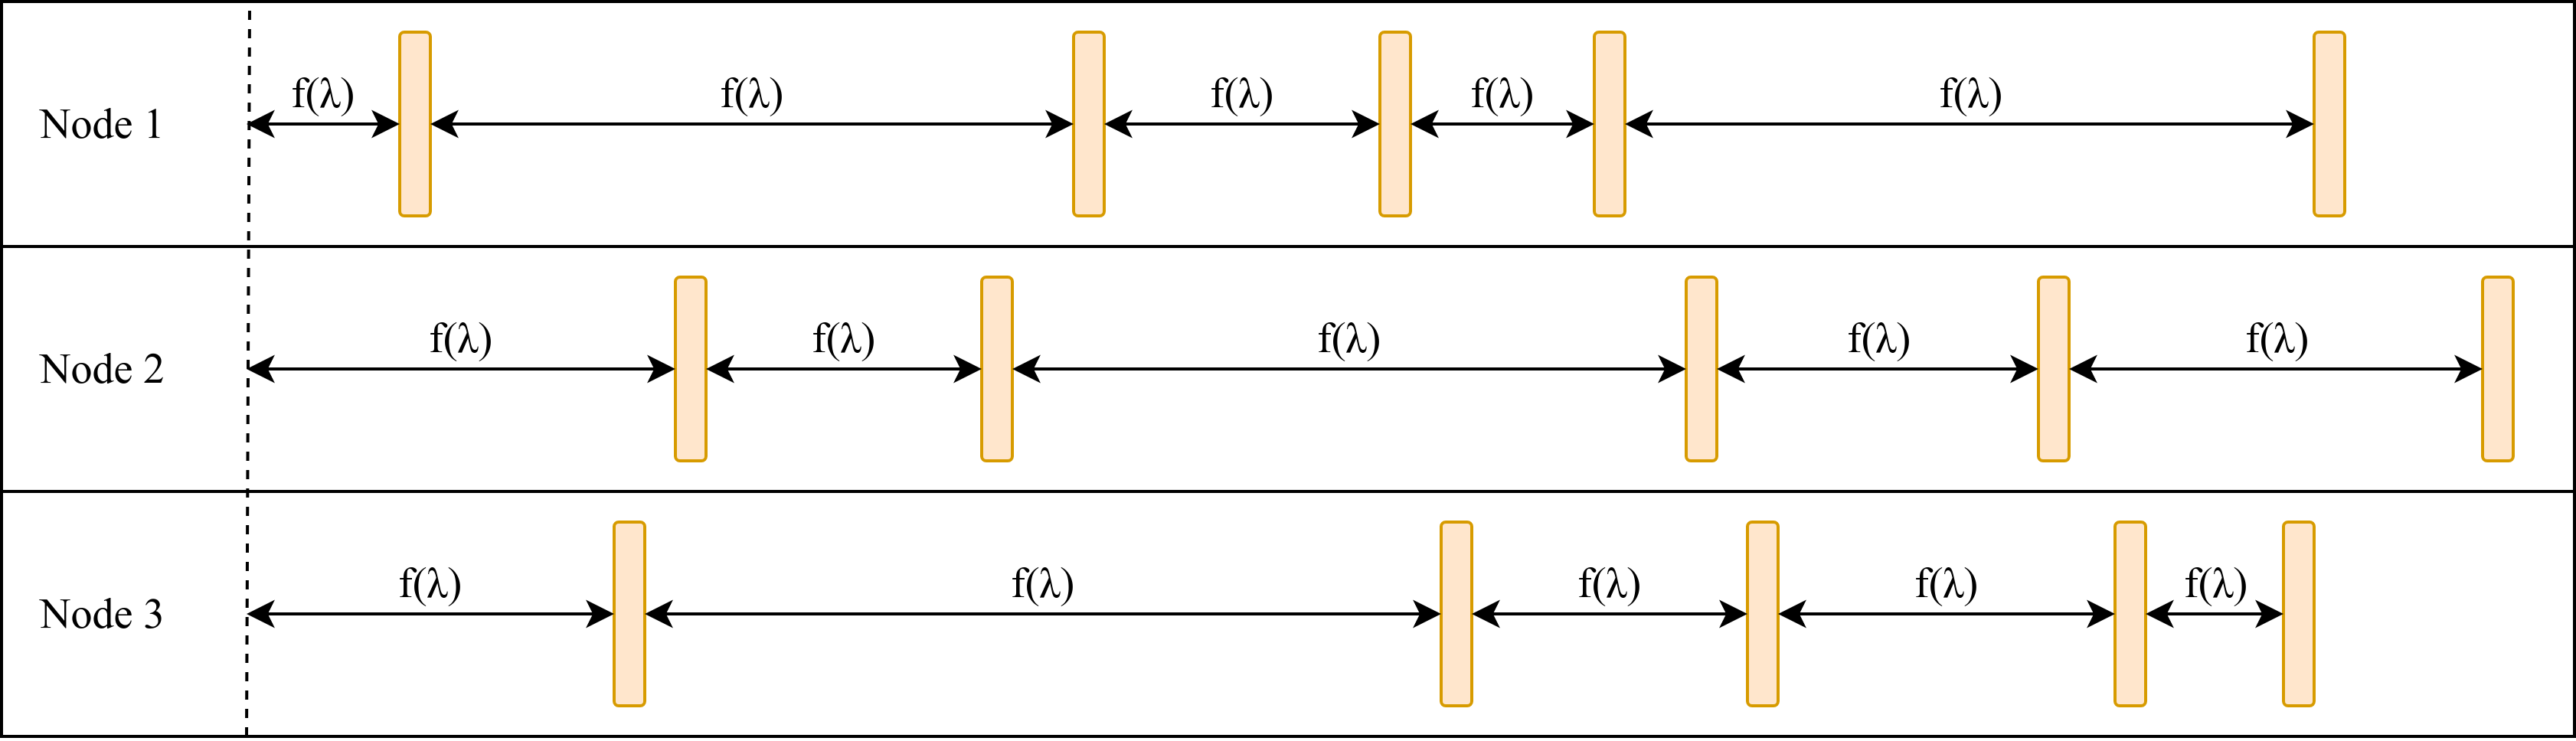
\includegraphics[width=\linewidth]{{fig/lora_traffic_poisson}.png}
\vspace*{2mm}
\caption{Poisson traffic generation timing diagram.}
\label{fig:lora_traffic_poisson}
\end{figure}

Downlink transmissions are not considered. Downlink transmissions are rare in real world deployments since ISM band regulations dictate duty cycle transmission limit for all devices including gateways. 

\section{Link Model Employed}

Link quality of a wireless system can be expressed by the metric of link budget. Link budget is a measure of all gains and losses from transmitter device to receiver device. Link budget of a wireless link can be calculated as \cite{AN1200.22}:

\begin{equation} \label{eq:expected_rx_power}
P^{dBm}_{RX} = P^{dBm}_{TX} + G^{dB}_{SYS} - L^{dB}_{SYS} - L^{dB}_{PATH}
\end{equation}

Where, $P^{dBm}_{RX}$ is the expected receive power at the receiver. $P^{dBm}_{TX}$ is the transmit power of the transmitter. $G^{dB}_{SYS}$ is the system gains such as transmitter and receiver antenna gains. $L^{dB}_{SYS}$ is the system losses such as transmitter and receiver line, circuit, antenna losses. $L^{dB}_{PATH}$ is the propagation path loss between transmitter and receiver antennas in open space. In the simulator, it is assumed that sum of system gains $G^{dB}_{SYS}$ and system losses $L^{dB}_{SYS}$ is +7 dB.

Maximum transmit power for European ISM band LoRa default channels can be found in Table \ref{table:max_tx_power}. In the simulator, it is assumed that nodes always select maximum allowed transmit power, which is 14 dBm. Different channel transmissions are independent from each other. However, this study focuses on spreading factor orthogonality. Thus, only single channel transmissions are utilized in the simulator.

\begin{table}
\centering
\caption{Gateway sensitivity for various spreading factors \cite{SX1276}.}
\label{table:gw_sf_sensitivity}
\begin{tabular}{|c|c|c|c|c|c|c|c|}
\hline
\multicolumn{2}{|c|}{\multirow{2}{*}{}} & \multicolumn{6}{c|}{\textbf{SF}} \\ \cline{3-8}
\multicolumn{2}{|c|}{}                  &    7 &    8 &    9 &   10 &   11 &   12 \\ \hline
\multirow{3}{*}{\textbf{BW (kHz)}}  & 125 & -123 & -126 & -129 & -132 & -133 & -136 \\ \cline{2-8}
                                    & 250 & -120 & -123 & -125 & -128 & -130 & -133 \\ \cline{2-8}
                                    & 500 & -116 & -119 & -122 & -125 & -128 & -130 \\ \hline
\end{tabular}
\end{table}

Receive sensitivity of a LoRa gateway for various spreading factors and bandwidths in dBm unit can be found in Table \ref{table:gw_sf_sensitivity}. In the simulator, 125 kHz bandwidth receive sensitivity values are used.

Free space propagation loss is calculated as \cite{TR136.942}:

\begin{equation} \label{eq:propagation_loss}
\begin{split}
P^{dB}_{PATH} = 40(1 - 4 \times 10^{-3} \times h){\log_{10} R|_{km}} \\
- 18 {\log_{10} h|_{m}} + 21 {\log_{10} f|_{MHz}} + 80
\end{split}
\end{equation}

Where, $h$ is the gateway altitude and $f$ is the frequency of the signal. In this work, it is assumed that $h$ = 15 m and $f$ = 868 MHz. With these assumptions, propagation loss calculation become \cite{7996384}:

\begin{equation} \label{eq:propagation_loss_simplified}
P^{dB}_{PATH} = 120.5 + 37.6 {\log_{10} R|_{km}}
\end{equation}

If the received signal power is higher than the gateway sensitivity, then signal can be decoded by the receiver successfully when there is no interfering transmission.

\section{Interference Model Employed}

In the simulator, interference model described in \cite{7996384} is adopted. They use SINR threshold matrix for modeling LoRa interference between simultaneous but different spreading factor LoRa transmissions.

In this work, it is assumed that there is no other technology interference in the network except LoRa interference. To exploit imperfect orthogonality of different spreading factor transmission, simulator should calculate the effect of different spreading factor transmissions to each other. In simulator, signal to interference plus noise ratio (SINR) threshold matrix $T_{i,j}$ from \cite{goursaud:hal-01231221} is used:

\begin{equation} \label{eq:sinr}	
T = \begin{bmatrix}	
       6 & -16 & -18 & -19 & -19 & -20 \\	
     -24 &   6 & -20 & -22 & -22 & -22 \\	
     -27 & -27 &   6 & -23 & -25 & -25 \\	
     -30 & -30 & -30 &   6 & -26 & -28 \\	
     -33 & -33 & -33 & -33 &   6 & -29 \\	
     -36 & -36 & -36 & -36 & -36 &   6	
     \end{bmatrix}	
\end{equation}

To decide if a referenced signal is interfered at receiver by an interfering signal, SINR threshold matrix is used. $T_{i,j}$ is SINR margin in dB unit between referenced signal with SF = i and interfering signal with SF = j to correctly decode the referenced signal. If there are more than one interfering signal, referenced signal must satisfy the margin for cumulative sum of all interfering signal received power for each spreading factor \cite{7996384}. SINR threshold can be calculated as:

\begin{equation} \label{eq:sinr_db}
SINR_{i,j} = \dfrac{P_{rc,0}}{\sum_{l \in I_j} P_{rc,l}}
\end{equation}

Where $P_{rc,0}$ is received signal power of referenced signal and $P_{rc,l}$ is received signal power of interfering signal for SF = j. If a packet with SF = i satisfies the following condition for every SF = j, then packet is survived from all interferences.

\begin{equation} \label{eq:sinr_t}
SINR_{i,j}^{dB} > T_{i,j}
\end{equation}

To calculate interfering power at receiver, we should consider the case where two transmissions are not perfectly overlapping. To equalize the interfering power at receiver \cite{7996384}:

\begin{equation} \label{eq:p_interference}
P_{rc,y}^{interf} = \dfrac{P_{rc,y}(t_{interf})}{t_{x}}
\end{equation}

Where $t_{x}$ is transmission duration of referenced signal. $t_{interf}$ is overlapping duration between referenced signal and interfering signal. Transmission duration of a packet can be calculated by data rate $R_{b}$ and packet size $PS$. Data rate of a LoRa transmission is already expressed in Equation \ref{eq:bit_rate_sf}. Duration of a LoRa transmission can be calculated as:

\begin{equation} \label{eq:transmission_duration}
t_{x} = \dfrac{8 \times PS|_{B}}{R_{b}|_{bps}}  \ s
\end{equation}

\section{Software}

The discrete event simulation tool is developed entirely with Python from scratch. The tool provides framework for simulating LoRaWAN networks. The tool keeps an transmission queue. Every event in this queue is a transmission. Every transmission has time, spreading factor, source, size, duration, and status fields. Every node generate an event according to their traffic generation rate parameter and inserts this event to simulation event queue. Initially all events are in pending state. Simulation tool then iterates and executes events, then marks events status as transmitted, interfered or under sensitivity. After all events are executed, the tool calculates network PDR, throughput and transmit energy consumption.

A command line parser is provided for interacting with the framework, this enables users to play with it without any programming or scripting. Also, an example script is provided to demonstrate usage of the framework. Python scikit-learn machine learning library is utilized for smart spreading factor schemes operations. Also, Python matplotlib library is used to generate figures in this thesis.

Source files of the simulation tool and their primary objectives are described below:

\begin{itemize}
  \item \textbf{main.py} \\ Command line interface of the simulator. It parses simulation inputs, executes simulation and reports simulation results.
  \item \textbf{simulation.py} \\ Core simulation methods and classes are defined. 'run' method is the core function that executes simulation steps.
  \item \textbf{packet.py} \\ LoRa related packet information classes are defined. Methods for calculating transmission duration, receive sensitivity, propagation loss and transmission energy are in this file. Also SNIR matrix and packet status enumeration types resides in this file.
  \item \textbf{node.py} \\ End node and gateway related classes are defined. Also, node traffic generator methods are defined.
  \item \textbf{topology.py} \\ LoRaWAN network topology information such as node and gateway locations are defined. Also, random topology generator method is defined.
  \item \textbf{location.py} \\ Location class that keeps x and y coordinate of nodes or gateways are defined.
  \item \textbf{paper.py} \\ An example application code for utilizing LoRa spreading factor simulation Python framework. This example script generates figures and results in this thesis.
\end{itemize}

Relationships between these classes can be seen in UML class diagram shown in Figure \ref{fig:uml_class}.

\begin{figure}
\centering
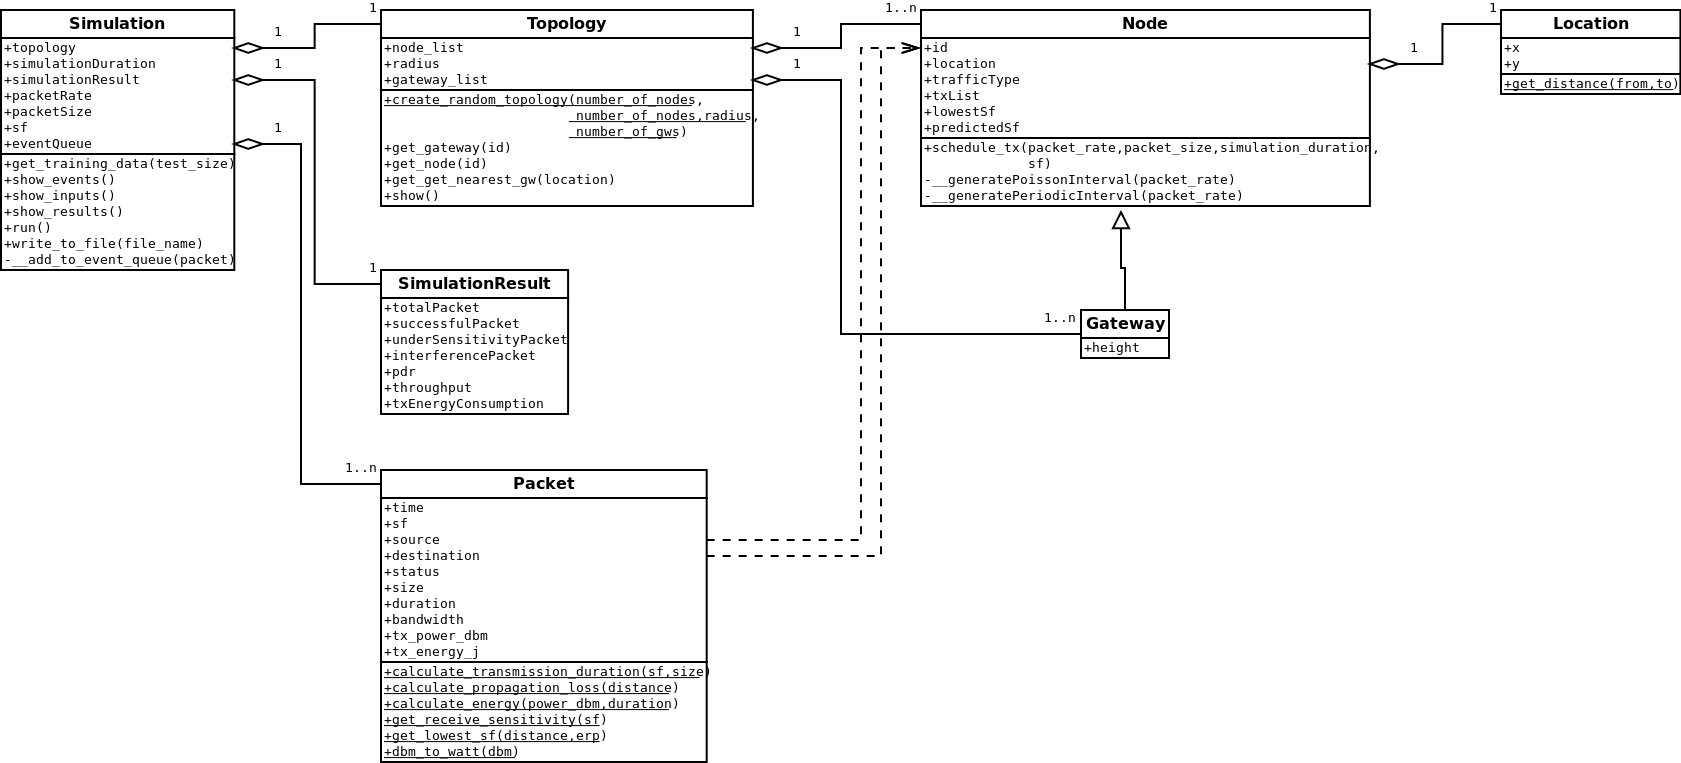
\includegraphics[scale=0.4,angle=90]{{fig/uml_class}.png}
\vspace*{5mm}
\caption{UML class diagram.}
\label{fig:uml_class}
\end{figure}

\subsection{Installation}

The simulation tool is developed and tested with Python 3.x \cite{python}.

The simulation tool requires specific Python modules to run. All of these modules can be installed by "pip" Python package manager. A new Python module can be installed with "pip install" command. Required Python modules for the simulation tool are:

\begin{itemize}
  \item matplotlib
  \item numpy
  \item scipy
  \item scikit-learn
\end{itemize}

\subsection{Command Line Interface Usage}

Command line interface examples of the simulation tool are given below:

\begin{itemize}
  \item Show help:\mint{Python}|python3 main.py -h|
  \item Topology radius in meter:\mint{Python}|python3 main.py -r 5000|
  \item Number of gateways:\mint{Python}|python3 main.py -g 3|
  \item Number of nodes:\mint{Python}|python3 main.py -n 300|
  \item Spreading factor assignment method:\mint{Python}|python3 main.py -s SF_Lowest|
  \item Smart spreading factor assignment classifier:\mint{Python}|python3 main.py -s SF_Smart -c DTC|
  \item Simulation duration in second:\mint{Python}|python3 main.py -d 3600|
  \item Packet rate in packet per second:\mint{Python}|python3 main.py -p 0.02|
  \item Packet size in byte:\mint{Python}|python3 main.py -z 80|
  \item Proportions of different traffic generator type nodes:\mint{Python}|python3 main.py -o 0.8 0.2|
  \item Random number generator seed:\mint{Python}|python3 main.py -e 42|
  \item Events log path:\mint{Python}|python3 main.py -l events.txt|
  \item Verbose level:\mint{Python}|python3 main.py -v INFO|
  \item Complex example:\mint{Python}|python3 main.py -r 7000 -g 3 -n 300 -s SF_Lowest -d 3600|
  \item Get figures and results in this thesis:\mint{Python}|python3 paper.py|
\end{itemize}
